\documentclass[./00_PhotoBox.tex]{subfiles}
\graphicspath{{\subfix{./img/}}}
\begin{document}


\chapter{Software-Entwicklung}
Für die Steuerung der Kameras und die anschließende Berechnung des 3D-Modelles muss ein Betriebssystem für das Kamerasystem und eine entsprechende Schnittstelle zu einer SfM-Software geschaffen werden. Diese Entwicklung erfolgte hauptsächlich in Python in Form von Prototyping. Das Kapitel beschreibt die Anforderungen an die Software in \autoref{sec:Anforderungsanalyse}. Anschließend werden hieraus die Anwendungsfälle (\autoref{sec:Anwendungsfallmodellierung}) erarbeitet und abschließend die Implementation (\autoref{sec:Implementierung}) beschrieben.

\section{Anforderungsanalyse}
\label{sec:Anforderungsanalyse}

\subsection{Funktionale Anforderungen}
\begin{itemize}
    \item Die Kameras sollen zeitgleich auslösbar sein. Die Auslösung soll möglichst ver\-zögerungs\-frei erfolgen.
    \item Die Steuerung soll auch unabhängig von anderen Geräten möglich sein, beispielsweise per Tastensteuerung.
    \item Der Status des Systemes soll für den Nutzer erkennbar sein - auch ohne Anschluss eines Computers etc..
    \item Es sollen Passpunkte automatisch gefunden und und für die Bestimmung der äußeren Orientierung genutzt werden.
    \item Die Bilder sollen scharf und fokussiert sein.
\end{itemize}

\subsection{Schnittstellen}
\begin{itemize}
    \item Die Daten sollen intern gespeichert werden.
    \item Eine Speicherung auf tragbaren Speichermedien wie USB-Sticks soll möglich sein.
    \item Eine direkte Übertragung an SfM-Software soll möglich sein.
\end{itemize}

\subsection{Nicht-funktionale Anforderungen}
\begin{itemize}
    \item Die Erfassung soll ohne weitere Hardware möglich sein. Das System soll unabhängig von Netzwerkanschlüssen etc. sein.
    \item Alle Kommunikation soll über WLAN erfolgen.
\end{itemize}

\section{Anwendungsfallmodellierung}
\label{sec:Anwendungsfallmodellierung}

Entsprechend der benötigten Schritte aus \autoref{c:photogrammmetrie} und \autoref{img:ablauf} wurde die Anwendungsfälle, die die Benutzeroberfläche ermöglichen soll, im Anwendungsfall-Dia\-gramm in \autoref{img:anwendungsfall} zusammengetragen.

\begin{figure}[!htbp]
    \centering
    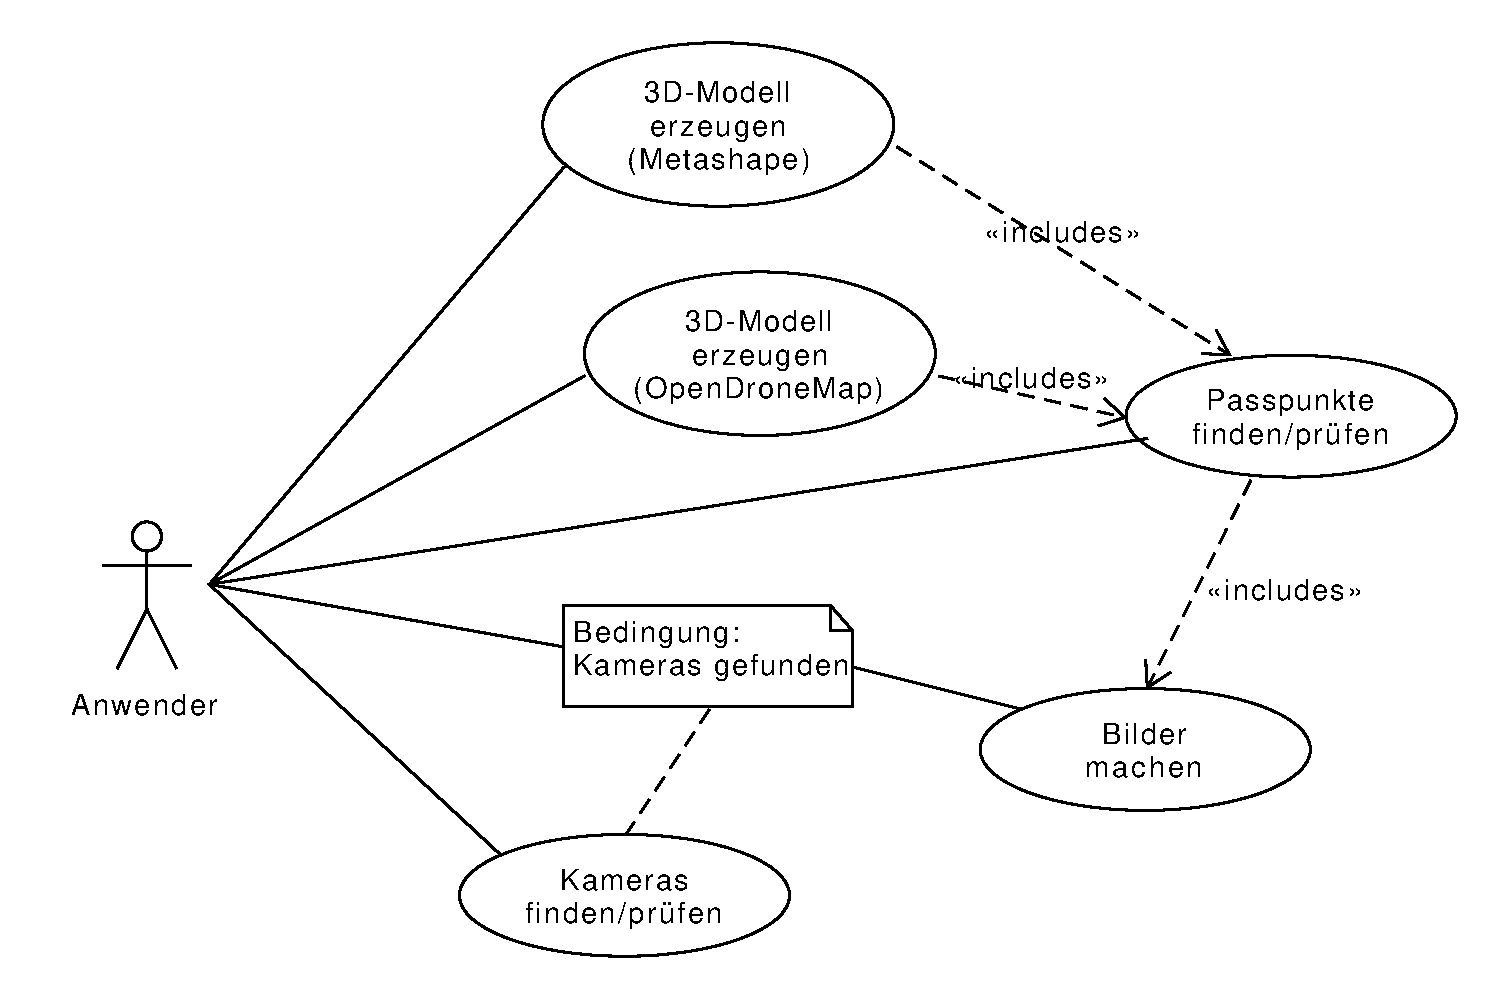
\includegraphics[width=1\textwidth]{./img/uml/uml_usecases.pdf}
    \centering
    \caption{Anwendungsfall-Diagramm} %Bildunterschrift
    \label{img:anwendungsfall} %ID fürs Bild
\end{figure}

Aus den benötigten Daten wurde das Domänen-Klassendiagramm aus \autoref{img:dokladia} erzeugt. Dieses zeigt vor allem die Abhängigkeiten der einzelnen Datensätze untereinander.

\begin{figure}[!htbp]
    \centering
    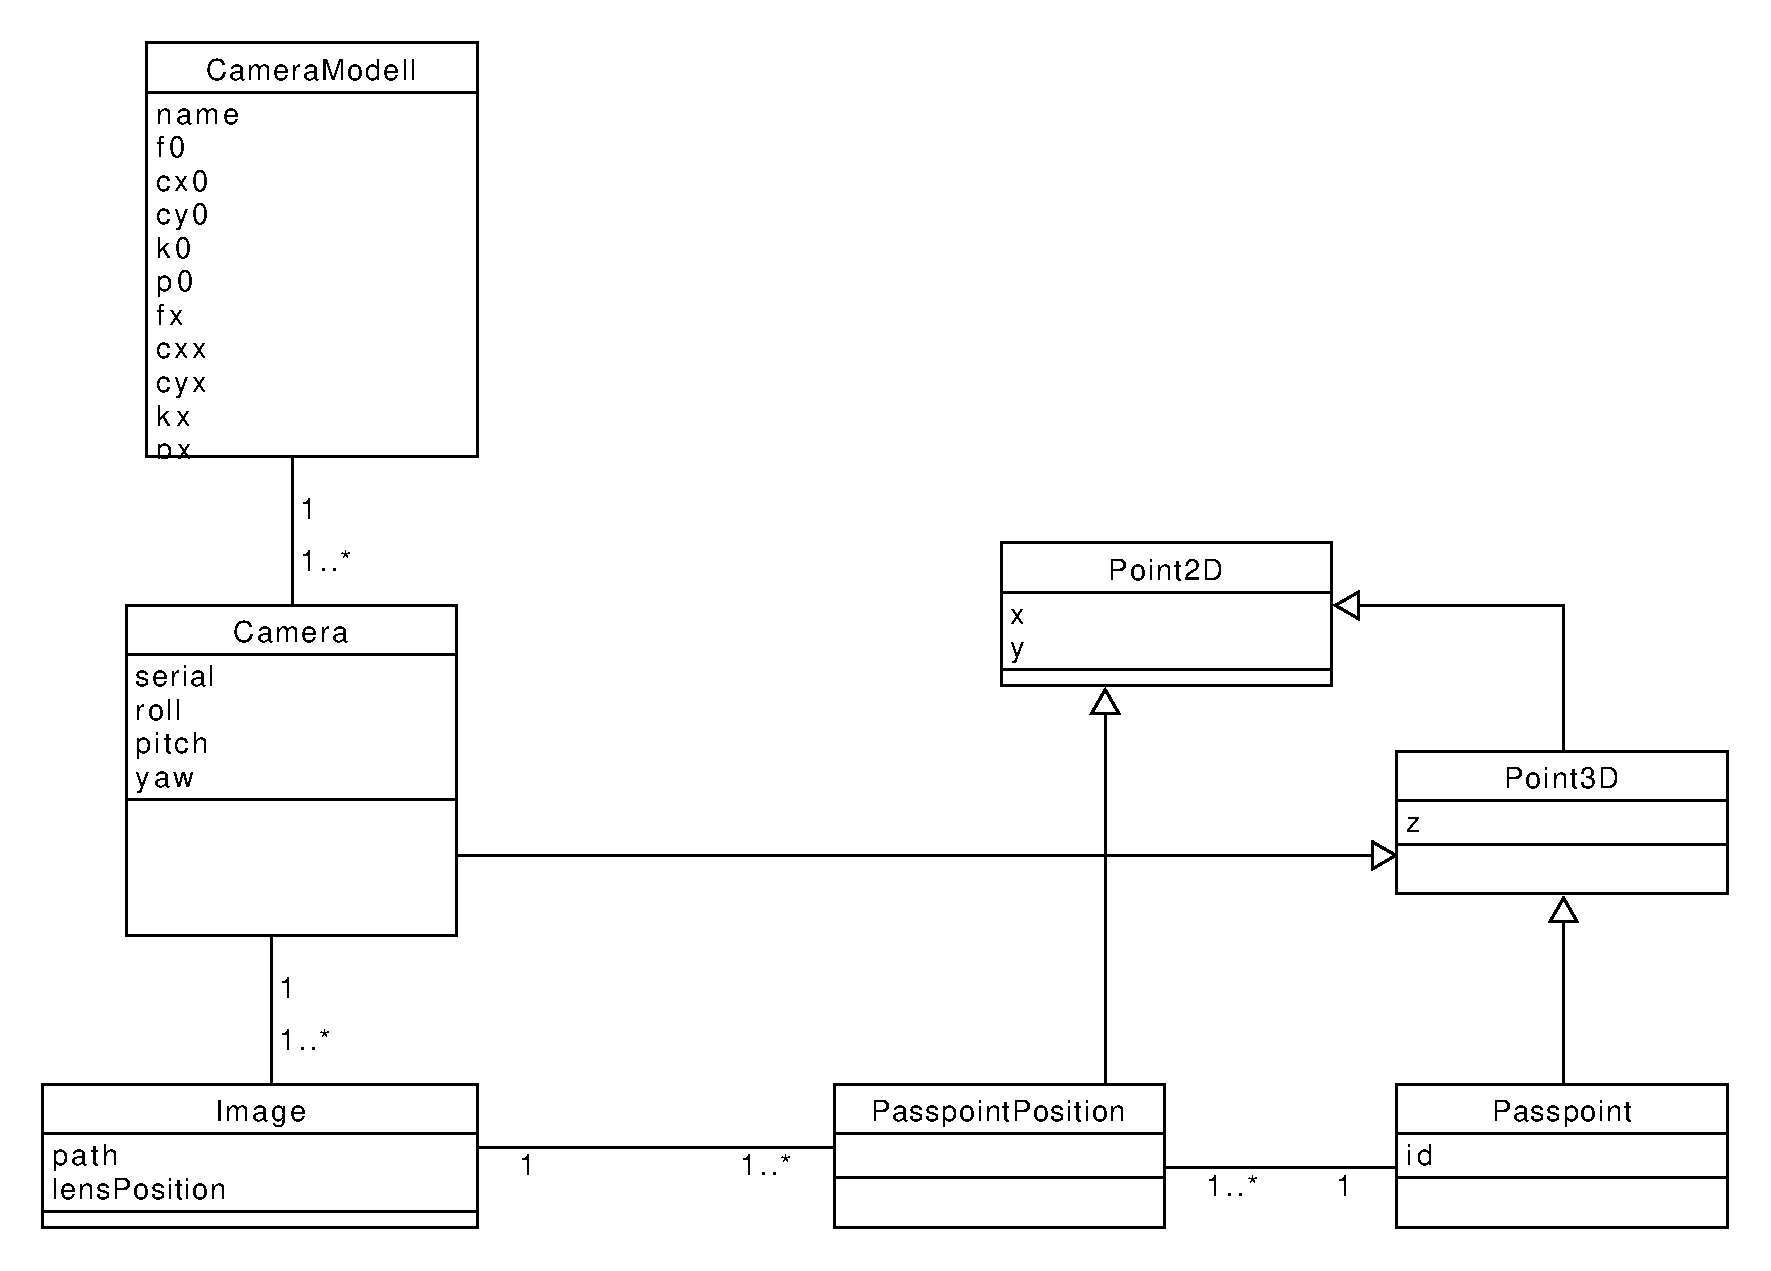
\includegraphics[width=1\textwidth]{./img/uml/uml_domain.pdf}
    \centering
    \caption{Domänen-Klassendiagramm} %Bildunterschrift
    \label{img:dokladia} %ID fürs Bild
\end{figure}

\section{Implementierung}
\label{sec:Implementierung}
Dieses ist dann auch Grundlage für die Implementierung der SQLite-Datenbank. Der Datenbankaufbau ist \autoref{img:datenbank} zu entnehmen. Die Datenbank dient der Zwischenspeicherung der Passpunkte und der durchgeführten Berechnungen.

\begin{figure}[!htbp]
    \centering
    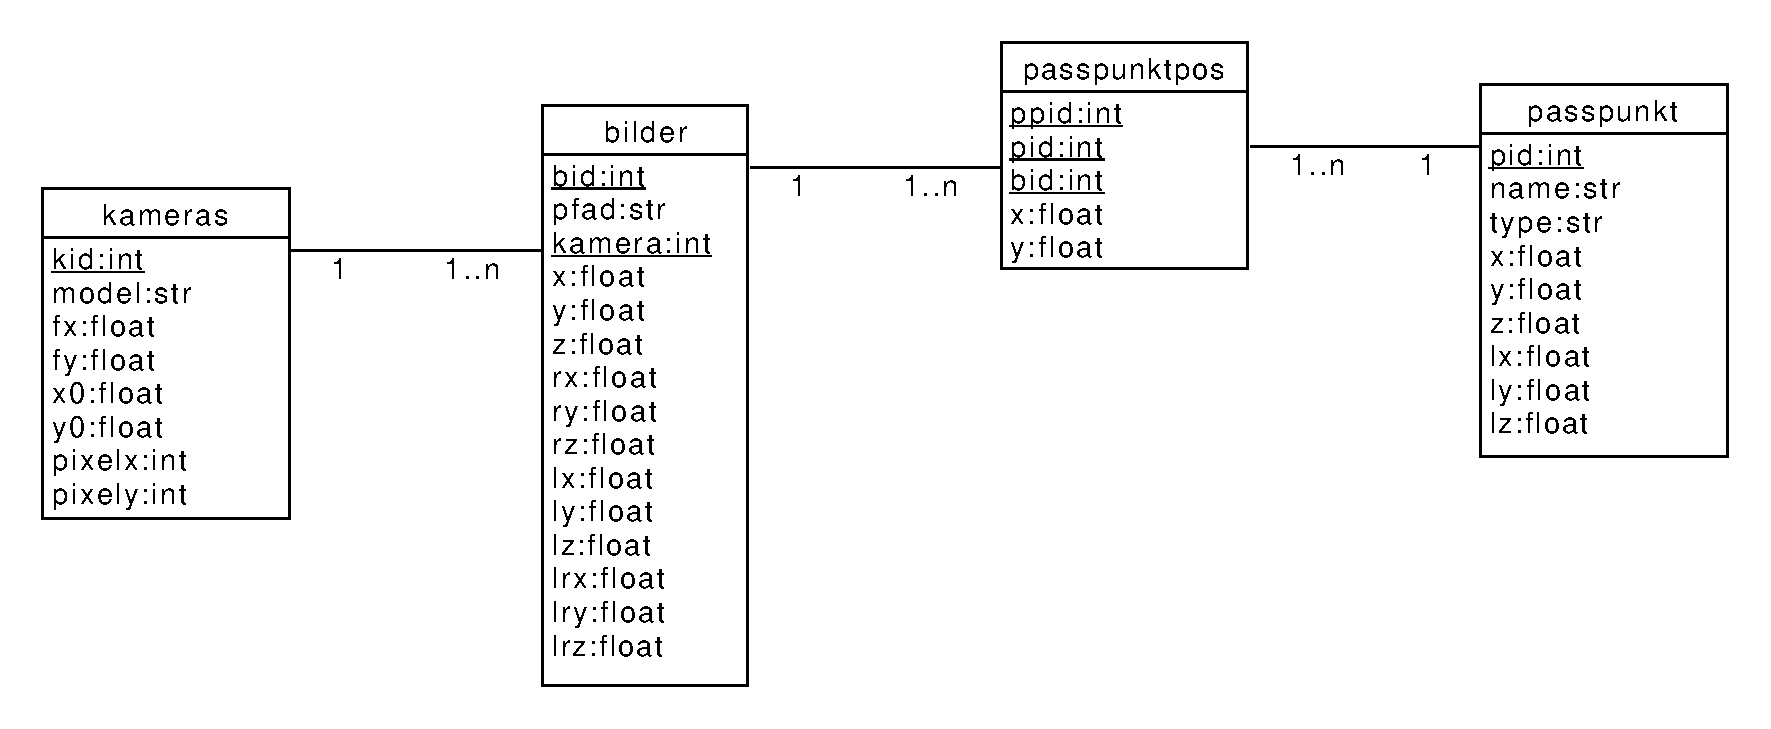
\includegraphics[width=1\textwidth]{./img/datenbank.pdf}
    \centering
    \caption{Datenbank-Struktur} %Bildunterschrift
    \label{img:datenbank} %ID fürs Bild
\end{figure}

Das Backend wurde in Python entwickelt. Die Pakete orientieren sich an den Arbeitsschritten aus dem Ablaufdiagramm (\autoref{img:ablauf}). Die einzelnen Python-Module greifen auf die oben beschriebene SQLite-Datenbank zu. Die einzelnen Module sind der Übersicht in \autoref{img:python} zu entnehmen.

\begin{figure}[!htbp]
    \centering
    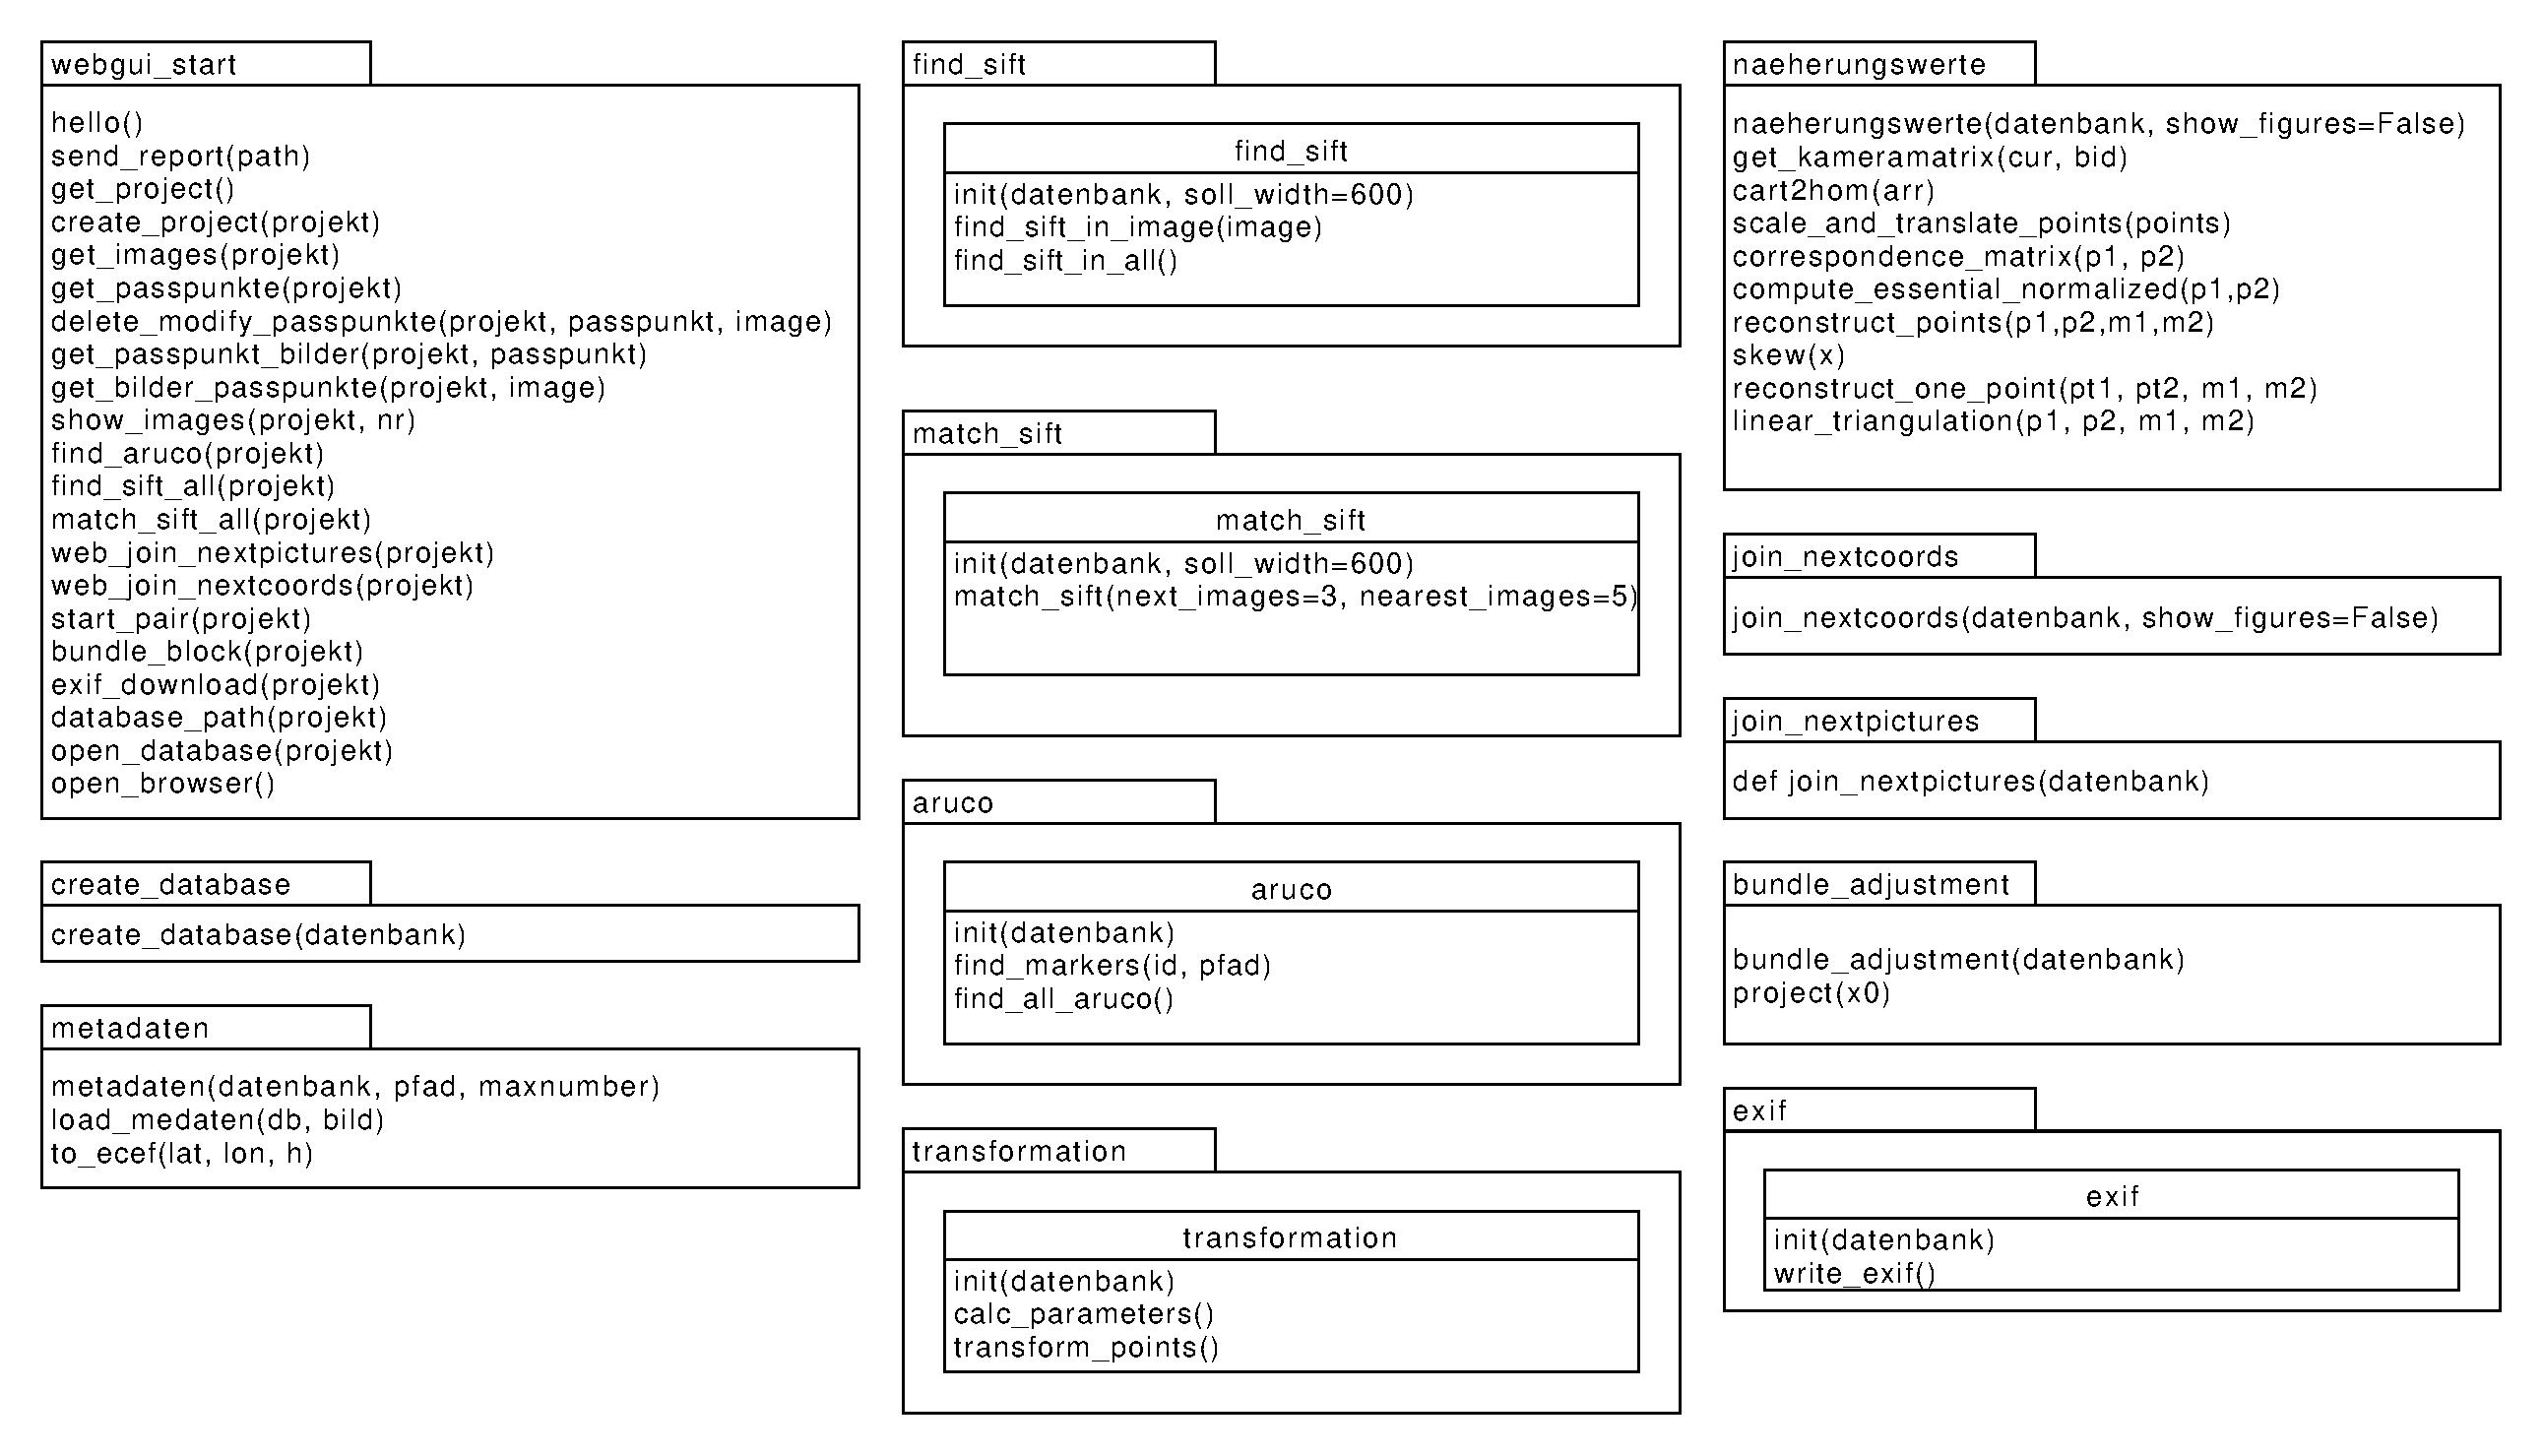
\includegraphics[width=1\textwidth]{./img/python.pdf}
    \centering
    \caption{Implementierung der Python-Pakete} %Bildunterschrift
    \label{img:python} %ID fürs Bild
\end{figure}

Über das Webstart-Modul werden dann die einzelnen Module über eine Website mit TypeScript angesprochen. Die einzelnen TypeScript-Klassen sind der \autoref{img:typescript} zu entnehmen. Hierbei wurde darauf Wert gelegt, die einzelnen Funktionen modular zu halten, sodass die Möglichkeit besteht, das System mit weiteren Modulen zu erweitern.

\begin{figure}[!htbp]
    \centering
    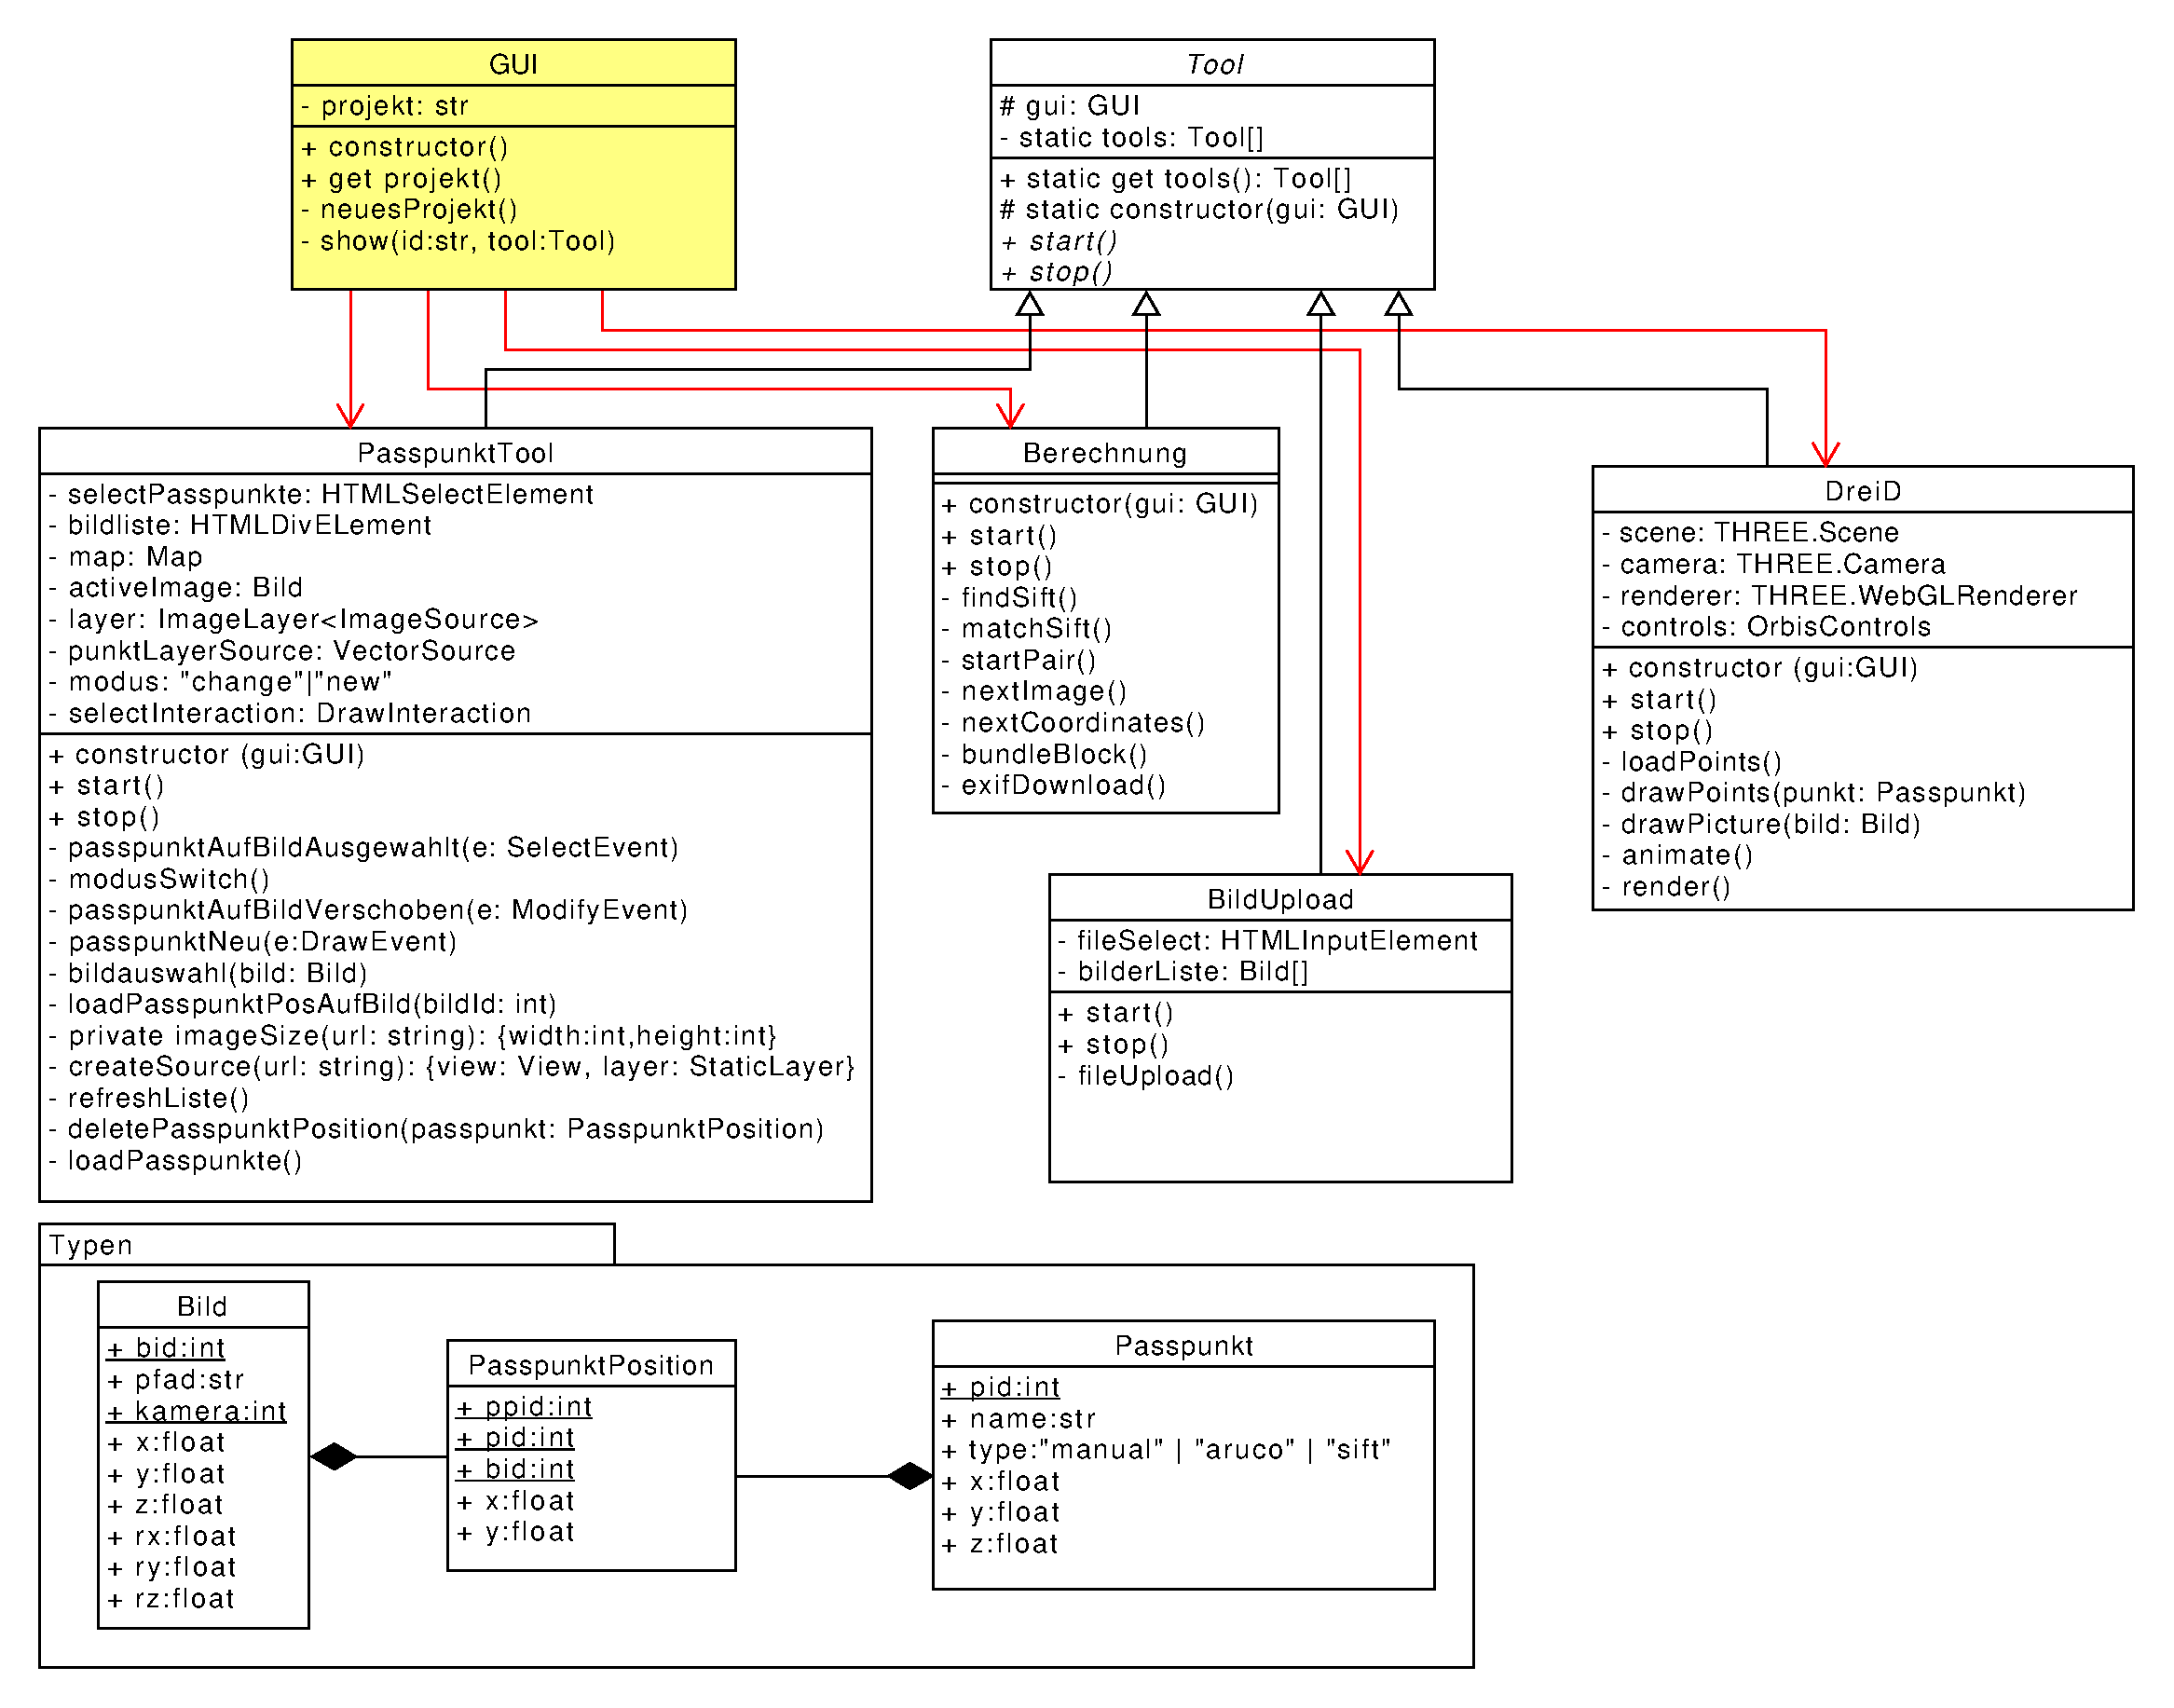
\includegraphics[width=1\textwidth]{./img/typescript.pdf}
    \centering
    \caption{Implementierung der TypeScript-Klassen} %Bildunterschrift
    \label{img:typescript} %ID fürs Bild
\end{figure}

\section{Untersuchungen}

\subsection{3D-Modell aus Fokusstacking}
\begin{itemize}
    \item Automatisierter Fokusstacking
    \item keine Beachtung der festen Ausrichtung
    \item Transformation über SIRF und Homographie
\end{itemize}


\subsection{Brennweitenänderung durch Fokussierung}
\begin{itemize}
    \item Charuco-Kalibriermuster
    \item Kamera und Board unbewegt
    \item 11 verschiedene Fokussierungen [0,5; 1; 2; 3; 4; 5; 6; 7; 8; 9; 10]
    \item Fokussierung nacheinander und 4 Wiederhoungen
    \item Erkennung des Musters
    \item Analyse der Unterschiede/Vergrößerung
\end{itemize}

\subsection{Änderung der Verzeichnung}
\begin{itemize}
    \item Kamera fest positioniert (keine Änderungen durch Schwerkraft)
    \item jeweils festen Fokus
    \item ChAruco-Board wird bewegt
\end{itemize}


\section{Vorgehen}
\label{ss:vorgehen}

Die Programmierung des Systemes erfolgte iterativ. Einzelne Arbeitspakete wurden in einem Jupyter-Notebook ausprobiert und dann, wenn dieser Schritt erfolgreich war, in den Gesamtworkflow integriert. Größtenteils wurden der Python-Code objektorientiert und typisiert geschrieben, einzelne Module sind jedoch noch aus der Prototyp-Phase funktionsbasierend programmiert.

\subsection{Python-Bibliotheken}
Es wurde, wenn möglich, auf Python-Bibliotheken zurückgegriffen. Hierdurch sollte der Programmieraufwand verringert und auf bereits getesteten Code gesetzt werden. Wo dieses nicht möglich war, wurden Funktionen entsprechend Code-Beispielen aus GitHub oder \glqq Rezepten\grqq{} aus dem Werk von \citeauthor{hartley} programmiert.

\subsubsection{OpenCV}
ist eine Bibliothek für Bildbearbeitung und maschinelles Sehen. Sie ist weit verbreitet und bietet viele photogrammetrische Funktionen. Viele der unter \autoref{s:photogramm} beschriebenen Schritte wurden mit dieser Bibliothek durchgeführt. \citep{opencv} Es zeigten sich jedoch Probleme bei der Berechnung der Essentiellen Matrix, sodass diese mit Hilfe eines Codebeispieles von \cite{3drec} auf Grundlagen von \cite{hartley} berechnet wurde.

\subsubsection{NumPy}
bietet neben vielen weiteren Funktionen die Möglichkeit der Matrizenrechnung. Diese wurde für viele Berechnungen benötigt.

\subsubsection{SciPy}
wurde für die Berechnung der Bündelblockausgleichung verwendet. Der manuelle Ansatz mit den Formeln aus \cite{luhmann4} unter Nutzung von NumPy war sehr ressourcenlastig. Unter Verwendung von SciPy und der Projektionsgleichung konnte die Berechnungsdauer stark dezimiert werden.

\subsubsection{Flask}
wurde genutzt um die Weboberfläche bereitzustellen und die Kommunikation zwischen dem Python und dem HTML/TypeScript-Modulen sicherzustellen. Die Weboberfläche selber muss nur einmalig kompiliert werden und wird dann von einen Flask-Webserver zur Verfügung gestellt. Per REST-Abfragen werden dann Daten zwischen TypeScript (bzw. nach dem Kompilieren eigentlich JavaScript) und Python ausgetauscht.

\subsubsection{OpenSFM}
wurde zwischenzeitlich verwendet um photogrammetrische Berechnung durchzuführen. Jedoch wurde dieses aufgrund mangelnder Anpassungsmöglichkeiten wieder verworfen. OpenSFM basiert aber auch unter anderem auf OpenCV. Der Code von OpenSFM wurde in der Prototyping-Phase zur Ideenfindung genutzt.

Erstaunlicherweise wurde kein brauchbares Paket zur Durchführung einer Helmert-Transformation mittels identischer Punkte gefunden. Daher wurde hier eine Funktion geschrieben, die eine Abbildungsmatrix mit Hilfe der Methode der kleinsten Quadrate errechnet. Nachteilig ist bei dieser Lösung jedoch, dass diese Ausgleichung auch Scherungen und unterschiedliche Maßstäbe für die einzelnen Koordinatenkomponenten unterstützt. Eigentlich wäre jedoch eine Transformation mit einem festen Maßstab sinnvoller, da die errechnete Struktur durch die Bündelblockausgleichung bereits deutlich besser der Realität entspricht als die GNSS-Koordinaten, die zur Transformation genutzt wurden. So werden die Daten aktuell an dieser Stelle wieder verschlechtert.

\subsection{TypeScript/JavaScript-Module}
Wie bereits erläutert wurde die GUI in Form einer Webseite entwickelt. Entsprechend wurden hier JavaScript-Module verwendet. Da TypeScript durch seinen Kompiler wieder zu JavaScript umgeformt wird, kann hier auch auf die große Auswahl von JavaScript-Bibliotheken aus dem Node Package Manager zurückgriffen werden.

\subsubsection{OpenLayers} ist eigentlich zur Anzeige von Online-Karten gedacht. In diesem Fall wurde es zur Darstellung der Passpunkte auf den Bildern genutzt. Es bietet einfache und weitläufig bekannte Funktionen zum Zoomen und Digitalisieren. Statt einer Karte wurde in dem entsprechenden Fenster das Bild und die Passpunkte als Marker auf diesem visualisiert. Auch die Editierfunktionen wurden hieraus genutzt.

\subsubsection{Three.JS} ist eine Bibliothek zur Darstellung von 3D-Inhalten. Diese wurde hier genutzt um eine Vorschau der errechneten 3D-Koordinaten bereitzustellen.


\end{document}